\section[Conclusiones]{Conclusiones y Trabajo a Futuro}
\begin{frame}{Conclusión}
    \begin{columns}
        \begin{column}{0.6\textwidth}
            \textbf{Durante la primera fase del Trabajo Terminal, se logró:}
            \begin{itemize}
                \item Establecer el planteamiento y la metodología que guiarán el desarrollo de la solución propuesta.
                \item Identificar diversos métodos y técnicas para abordar eficazmente la problemática planteada.
                \item Consultar a expertos para validar el enfoque y alinearlos con los objetivos del proyecto.
            \end{itemize}
        \end{column}
        \begin{column}{0.4\textwidth}
            % Aquí podrías incluir una imagen de ejemplo
            \centering
            \begin{figure}[H]
                \centering
                \adjustbox{max width=\textwidth, max height=0.5\textheight}{%
                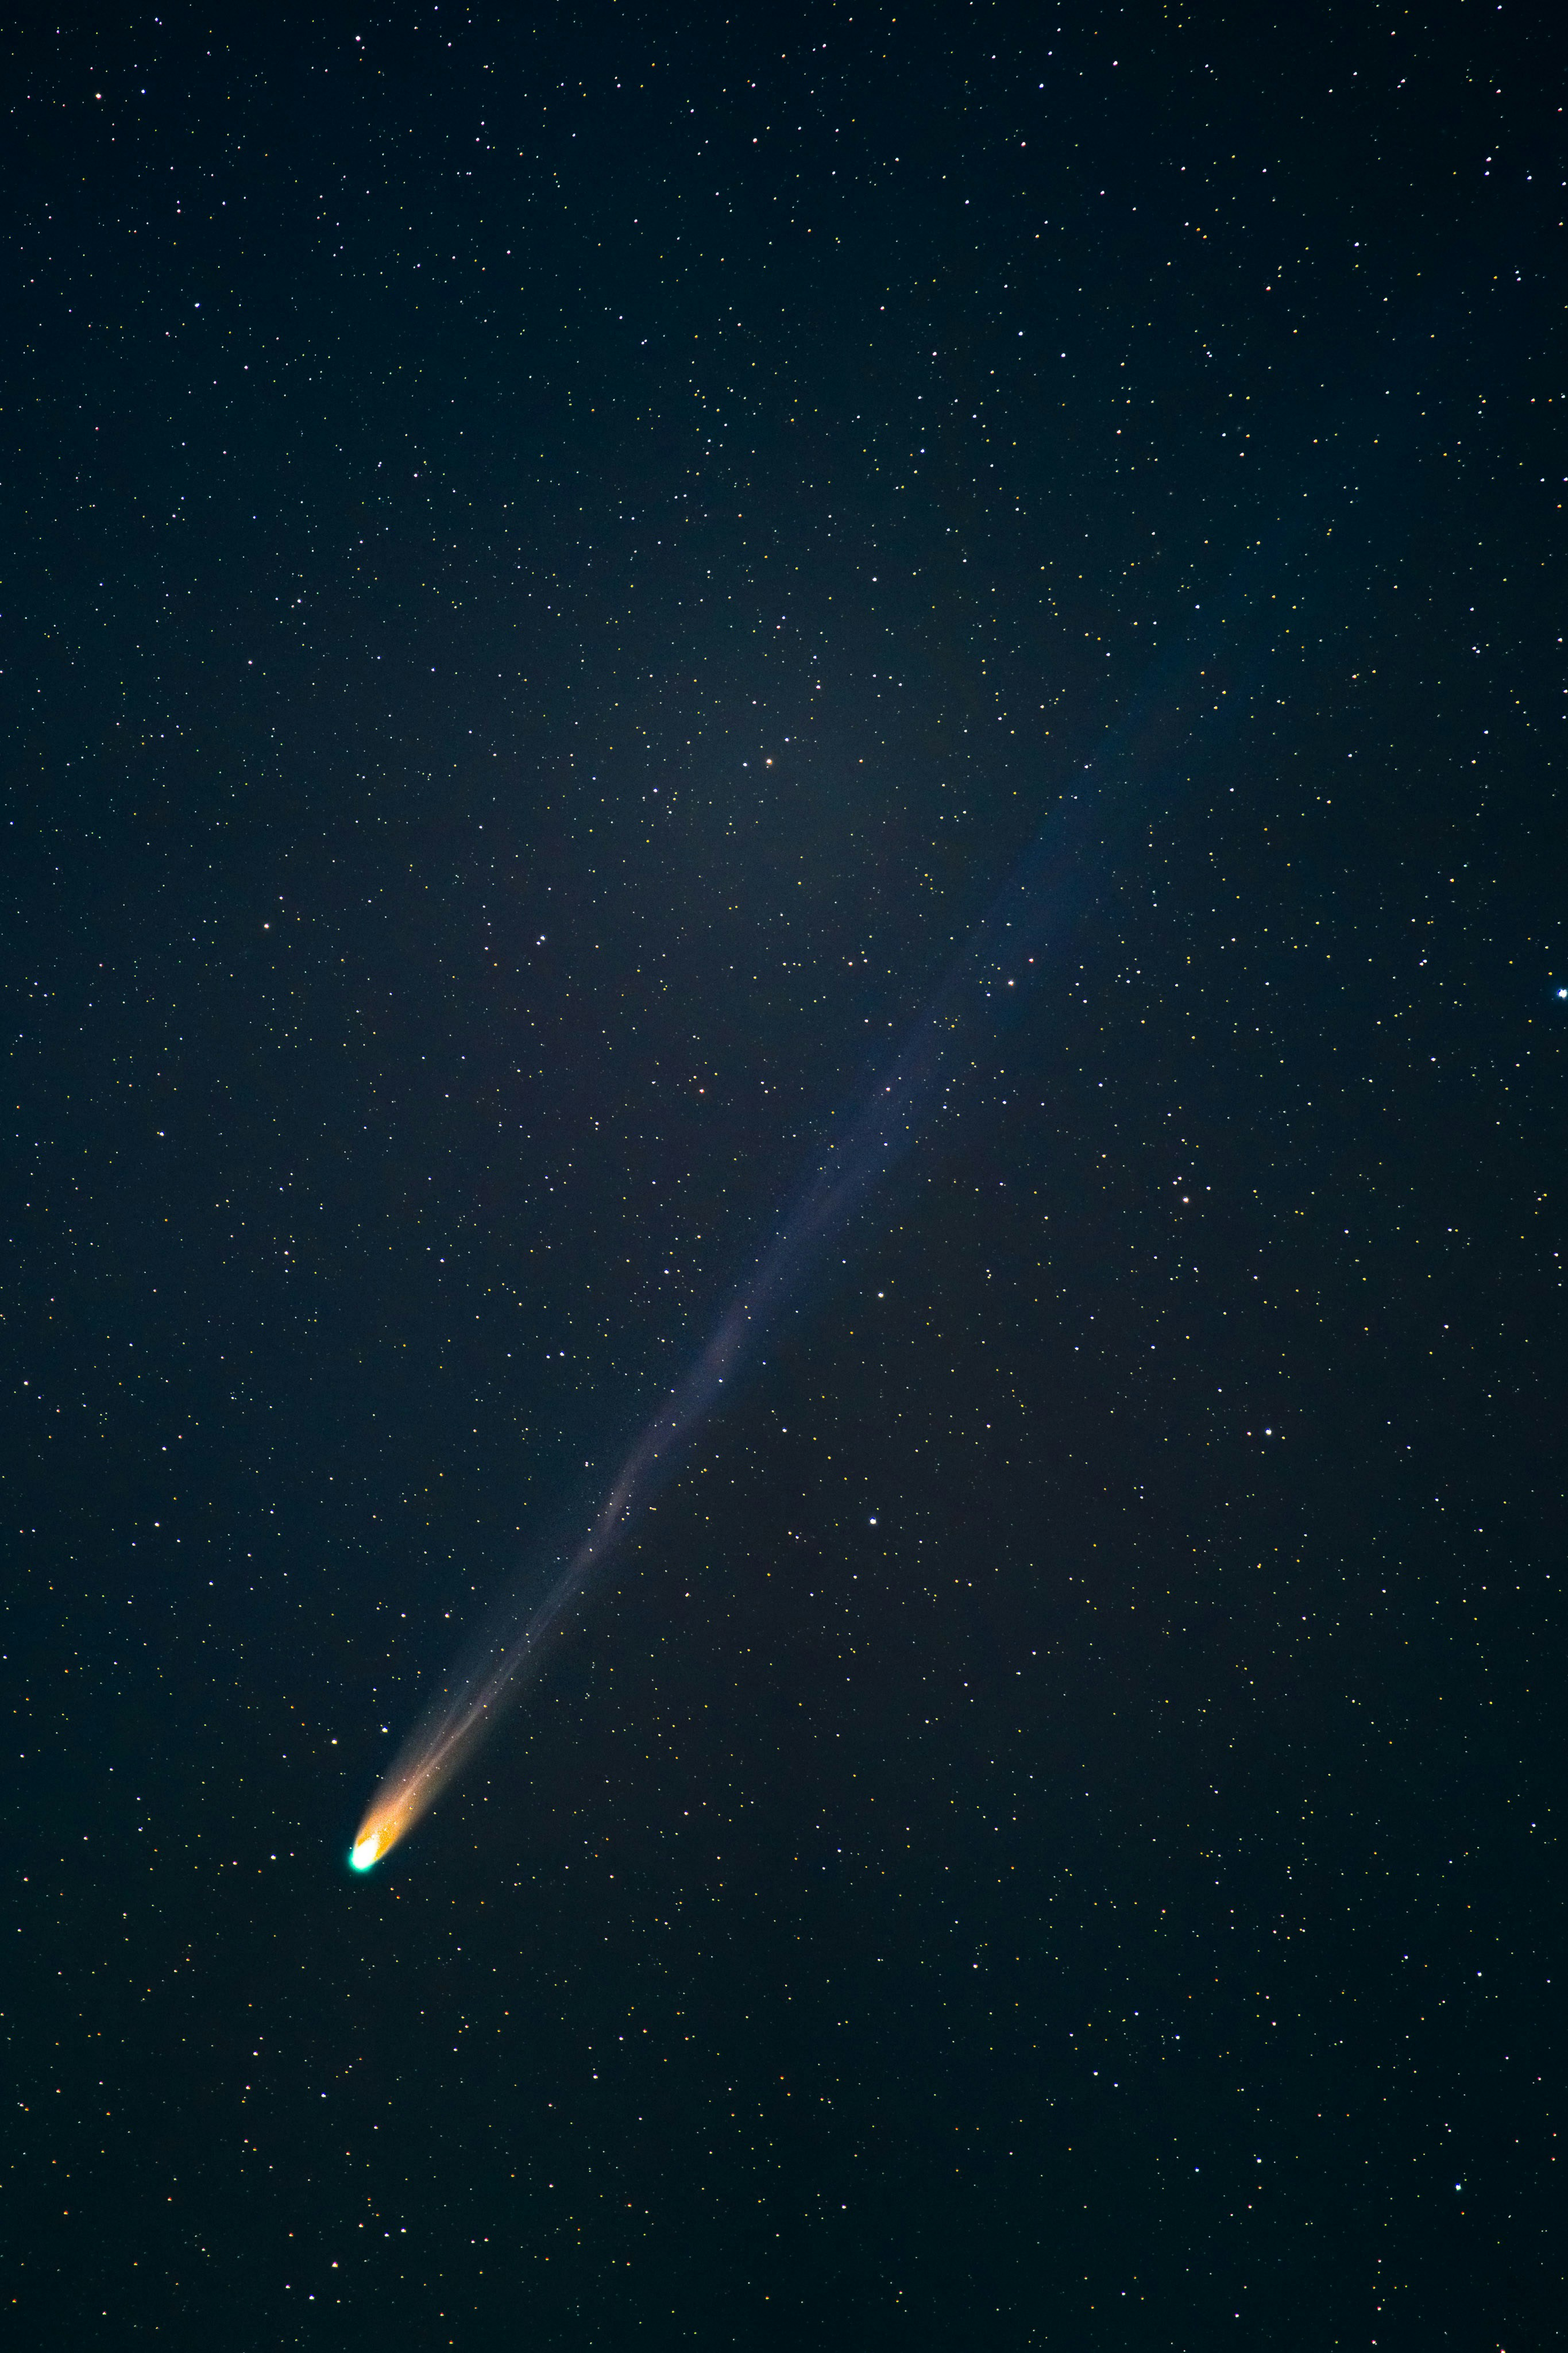
\includegraphics{img/conclusion/cometa.jpg}
                }
                \vspace{-0.25cm}
                \caption{\tiny~Una vista del cielo mirando hacia arriba por la noche \textit{Autoría de:}~\cite{dyer_cielo_nocturno_2021}}%
                \label{fig:Matplotlib_logo}
            \end{figure}
        \end{column}
    \end{columns}
\end{frame}

\begin{frame}{Pasos Iniciales}
    \begin{columns}[T] 
        \begin{column}{0.55\textwidth} 
            \begin{figure}
                \centering
                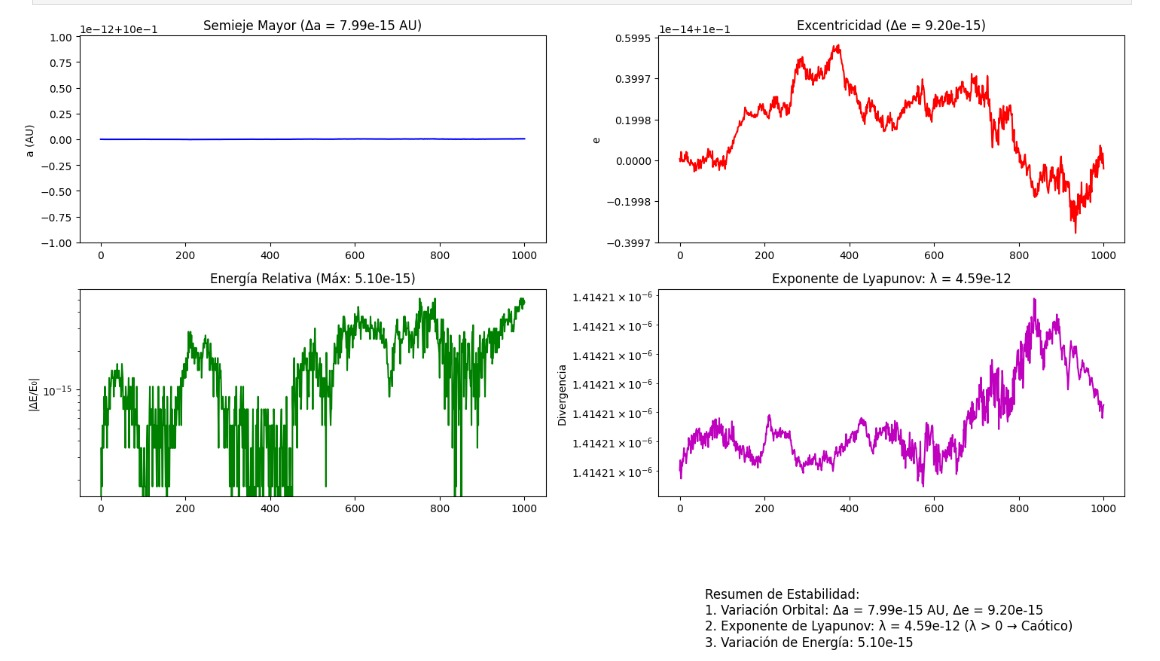
\includegraphics[width=\textwidth]{img/conclusion/metricas.jpeg} 
                \caption{Gráficas de estabilidad orbital.}
            \end{figure}
        \end{column}

        \begin{column}{0.38\textwidth} 
            \begin{figure}
                \centering
                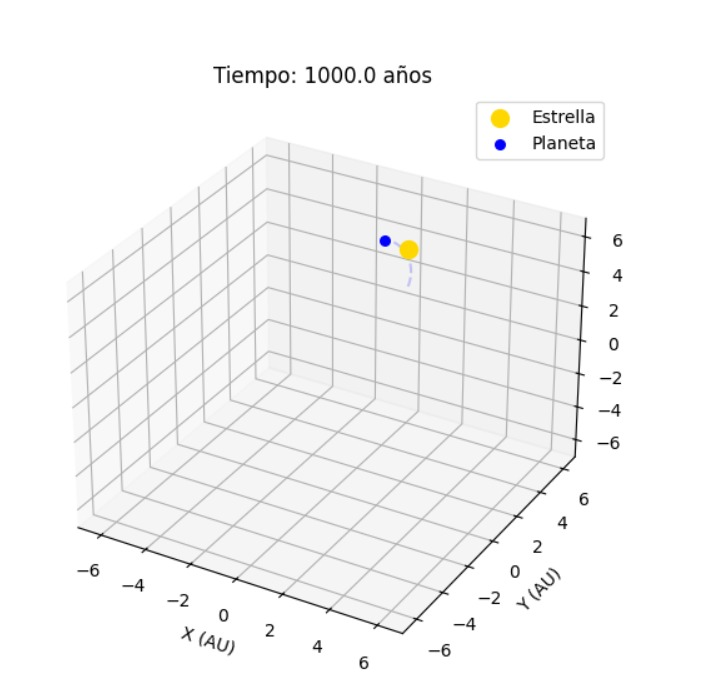
\includegraphics[width=\textwidth]{img/conclusion/simulacion.jpeg} 
                \caption{Representación 3D de una órbita.}
            \end{figure}
        \end{column}
    \end{columns}
\end{frame}


\begin{frame}{Trabajo a futuro}
    \begin{columns}
        \begin{column}{0.4\textwidth}
            % Aquí podrías incluir una imagen de ejemplo
            \centering
            \begin{figure}[H]
                \centering
                \adjustbox{max width=\textwidth, max height=0.5\textheight}{%
                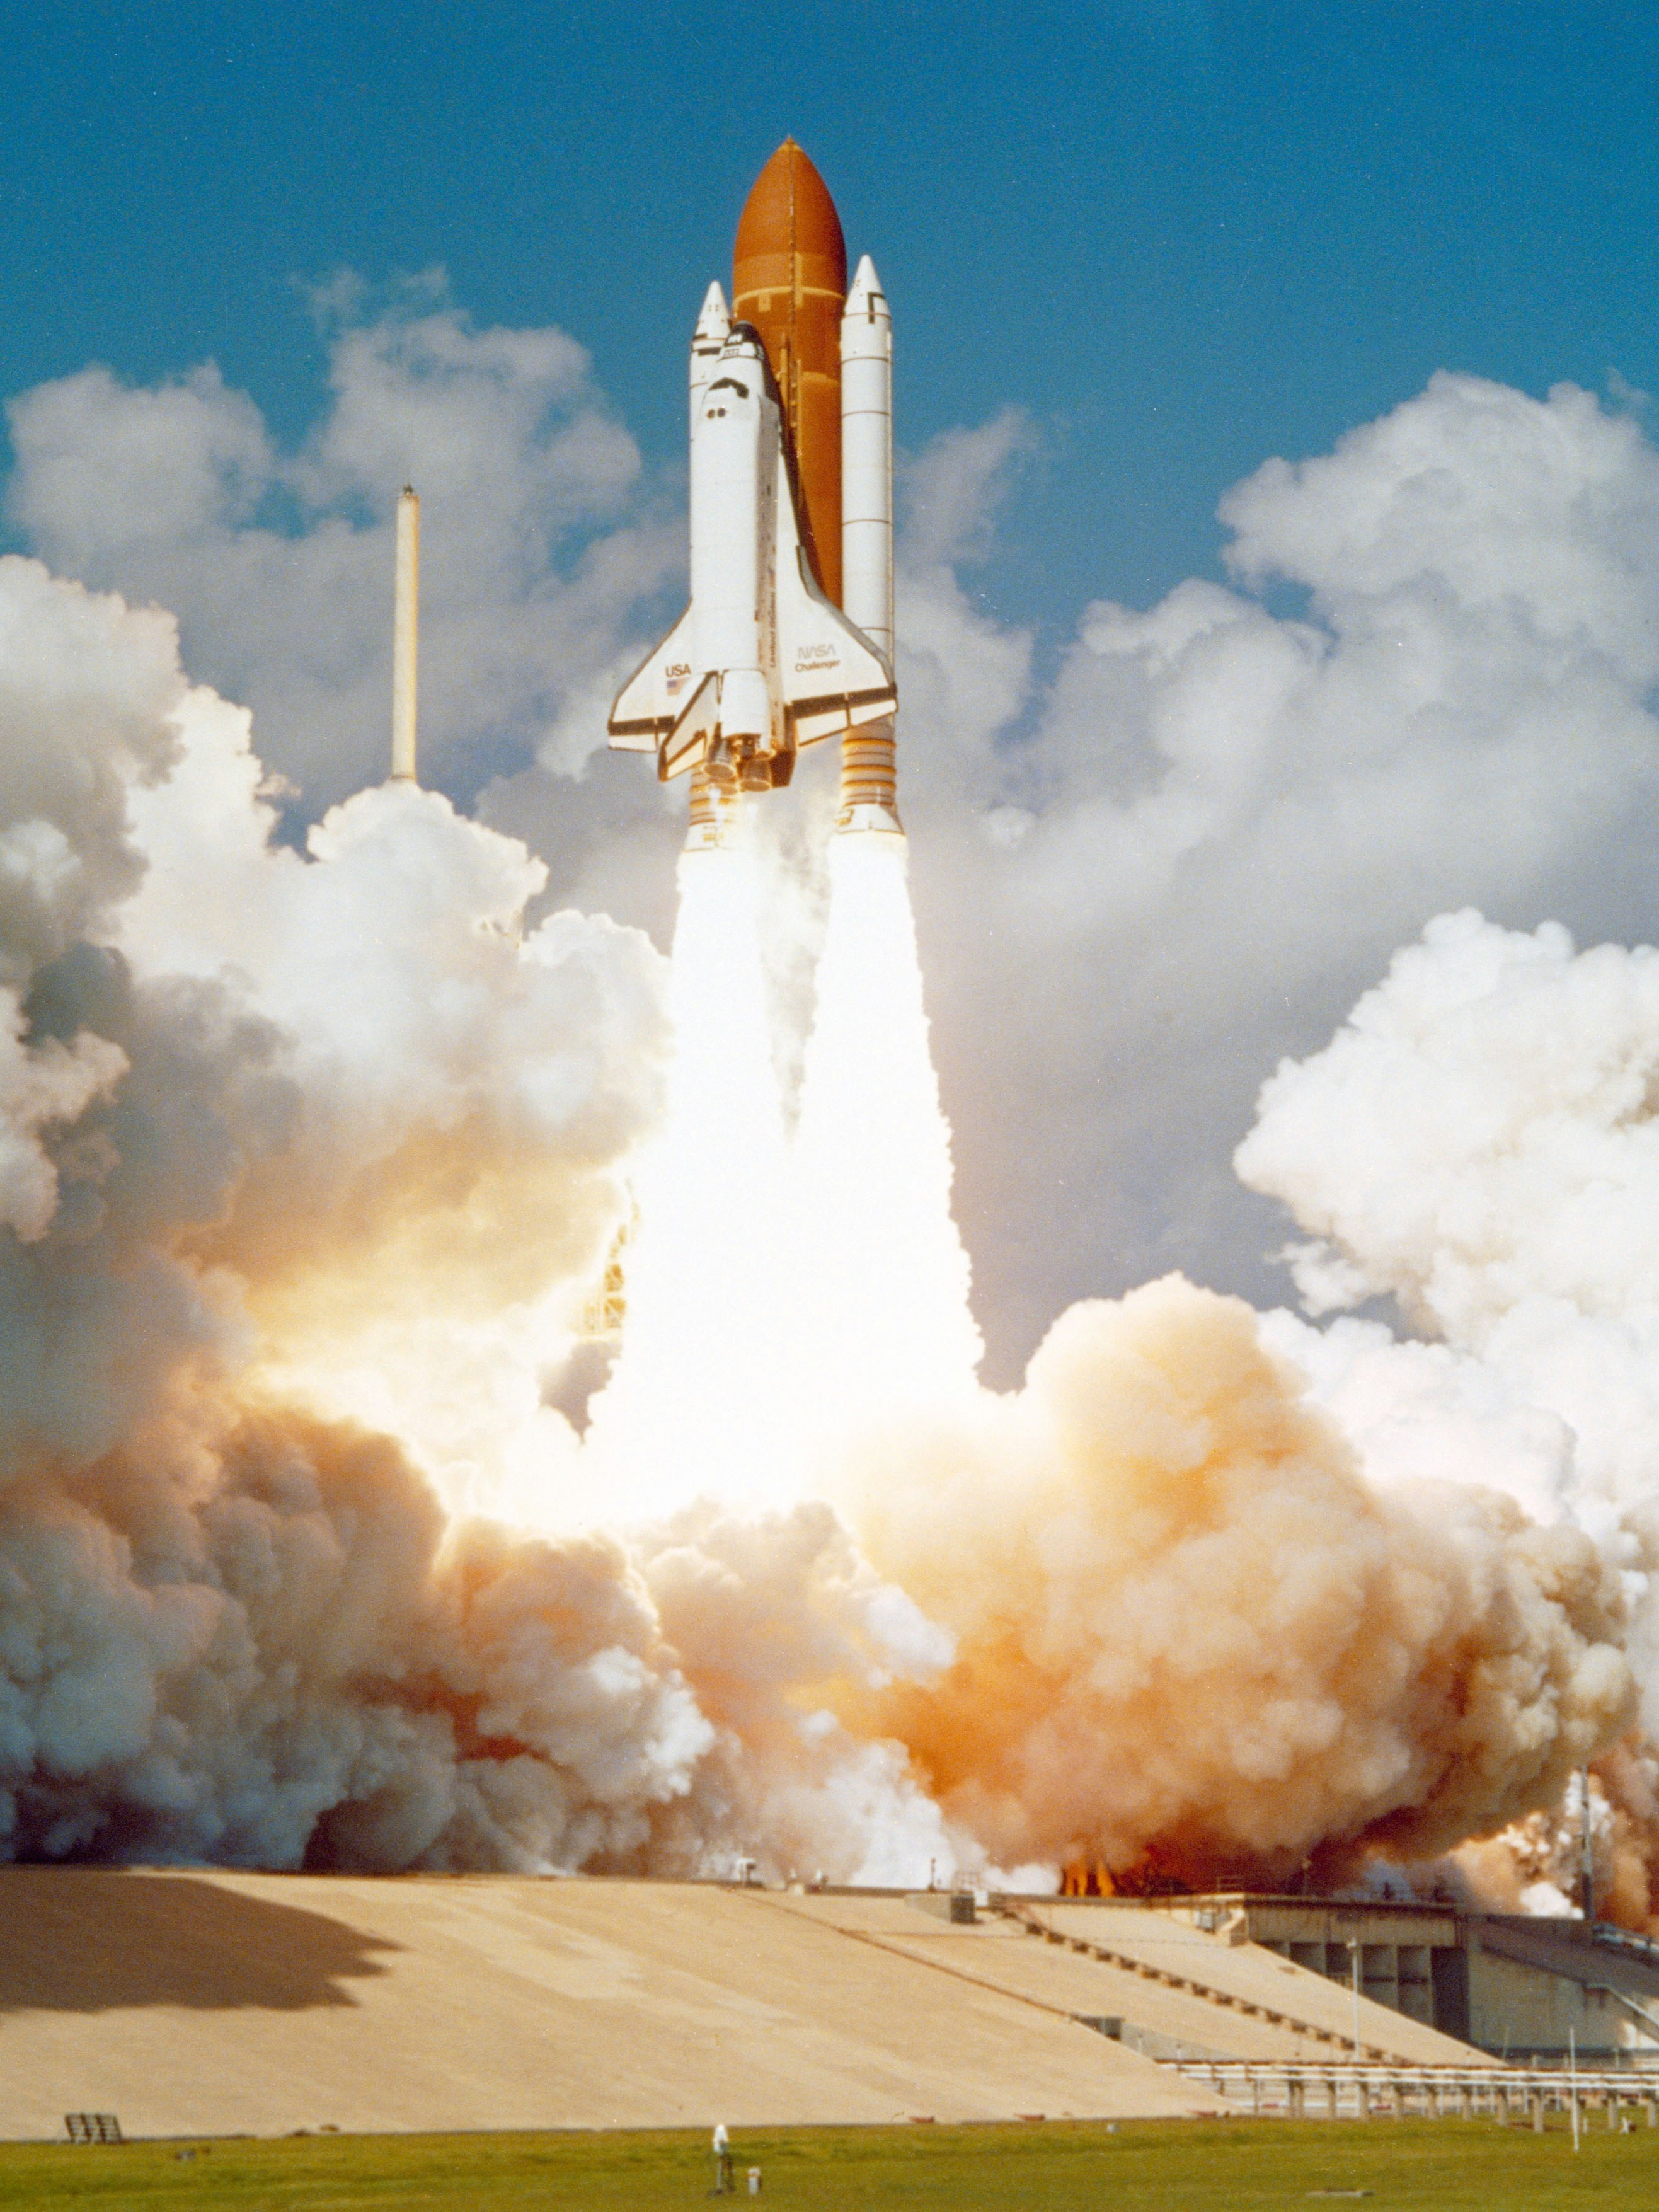
\includegraphics{img/conclusion/spaceshipNasa.jpg}
                }
                \vspace{-0.25cm}
                \caption{\tiny~Transbordador espacial Challenger se lanza desde el Centro Espacial Kennedy.~\textit{Autoría de:}~\cite{nasa_challenger_unsplash}}%
                \label{fig:PyQt_logo}
            \end{figure}
        \end{column}
        \begin{column}{0.6\textwidth}
            Para la siguiente fase del proyecto terminal, se realizarán las siguientes tareas:
            \begin{itemize}
                \item Desarrollo de pseudocódigos
                \item Implementación de módulos.
                \item Pruebas y refinamiento.
                \item Consulta con expertos y miembros del comité sinodal sobre los avances.
                \item Elaboración de un manual de usuario.
            \end{itemize}
        \end{column}
    \end{columns}
\end{frame}